\section{Tarea}

\subsection{Problema propuesto: }

\begin{enumerate}[label={[\arabic*]}]
    \item Usar clase template para implementar estructuras de lista enlazada simple & que permita armar secuencia de edades & secuencia de palabras. 
    \item Trascribir y analizar el siguiente código, describir el comportamiento.
    \item Crear una interface gráfica (que implemente señales y slots) que muestre una lista de países, al dar clic sobre alguno que se muestre un Label o Text con el idioma y capital correspondiente.
\end{enumerate}




\section{Equipos, materiales y temas utilizados}

\begin{itemize}
    \item Subsistema de Windows para Linux (WSL) con Ubuntu.
    \item Sistema operativo: Microsoft Windows [Versión 10.0.26100.6584]
    \item TeX Live 2025
    %\item Strawberry Perl (requerido por MiKTeX para la ejecución de scripts auxiliares en la compilación de ciertos paquetes).
    \item Helix 25.01.1 (e7ac2fcd)
    \item Visual Studio Code 1.104.0 x64
    \item Git version 2.41.0.windows.1
    \item Cuenta activa en GitHub para la gestión de repositorios remotos.
    \item Plantillas
    \item Leguaje de programación C++
    %\item Librería Qt
\end{itemize}




\section{URL de Repositorio Github}

\begin{itemize}
    \item URL del Repositorio GitHub para clonar o recuperar.
    \item \url{https://github.com/yhuayhuahi/Teo.git}
    \item URL para el laboratorio (\itemPracticeNumber) en el Repositorio GitHub.
    \item \url{https://github.com/yhuayhuahi/Teo/tree/main/laboratorios/lab\itemPracticeNumber}
\end{itemize}




\section{Desarrollo de las actividades}

\subsection {\textcolor{red}{Actividad 01: Implementación en C++ pata una lista enlazada simple}}

\subsubsection {Función Main en C++}

A continuación se muestra la implementación de la función main en C++ para probar la clase template de una lista enlazada simple que permite armar secuencias de enteros para este caso.

\begin{lstlisting}[style=cpp-style, caption={Función Main en cpp}]
#include <iostream>
#include "cola.h"

using namespace std;

int main() {
    // Probar con enteros
    Cola<int> cola;
    
    cola.insertarValor(10);
    cola.insertarValor(20);
    cola.insertarValor(30);
    
    cout << "Cantidad: " << cola.accederCantidad() << endl;
    cola.mostrarCola();
    
    // Buscar y eliminar
    cola.eliminarValor(20);
    cout << "Después de eliminar: " << cola.accederCantidad() << endl;
    cola.mostrarCola();
    
    return 0;
}
\end{lstlisting}

La implementación de la clase template Cola se encuentra en el archivo cola.h que se adjunta en el repositorio del laboratorio.

\subsubsection{Prueba de ejecución}

Se realizo la prueba de ejecución del código en C++ y se obtuvo el siguiente resultado:

\begin{figure}[H]
    \centering
    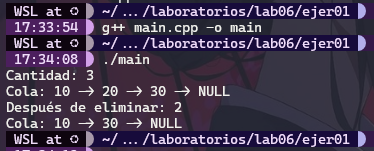
\includegraphics[width=0.5\textwidth]{img/Prueba01.png}
    \caption{Prueba de ejecución de la lista enlazada simple}
    \label{fig:qt_app}
\end{figure}




\subsection{\textcolor{red}{Actividad 02}}

Se tiene el siguiente código en C++, brindado en la guía de laboratorio:

\begin{lstlisting}[style=cpp-style, caption={Código en C++ brindado en la guía de laboratorio}]
#include <iostream>

using namespace std;

template <class T>
class Contenedor {
    T elemento;
public:
    Contenedor(T arg) { elemento = arg; }
    T add() { return ++elemento; }
};

template <>
class Contenedor <char> {
    char elemento;
public:
    Contenedor(char arg) { elemento = arg; }
    char uppercase ()
    {
        if ((elemento >= 'a') && (elemento <= 'z')) {
            elemento += 'A' - 'a';
        }
        return elemento;
    }
};

int main() {
    Contenedor<int> cint(5);
    Contenedor<char> cchar('t');
    std::cout << cint.add() << std::endl;
    std::cout << cchar.uppercase() << std::endl;
    return 0;
}
\end{lstlisting}

\subsubsection{Análisis del código}

El código presentado define una clase plantilla `Contenedor` que puede almacenar un elemento de cualquier tipo. Se proporciona una especialización para el tipo `char` que incluye un método para convertir el carácter a mayúsculas. En la función `main`, se crean instancias de `Contenedor` para un entero y un carácter, y se muestran los resultados de las operaciones. \\

Al ejecutar el código, se observa que la instancia de `Contenedor<int>` incrementa el valor entero de 5 a 6, mientras que la instancia de `Contenedor<char>` convierte el carácter 't' a su equivalente en mayúscula 'T'. Por lo tanto, la salida del programa será:

\begin{figure}[H]
    \centering
    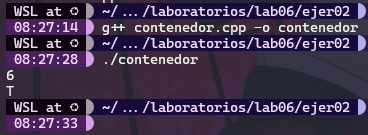
\includegraphics[width=0.5\textwidth]{img/Prueba02.png}
    \caption{Salida del programa al ejecutar el código proporcionado}
\end{figure}

Esto demuestra el uso de plantillas en C++ para crear clases genéricas y la capacidad de especializar comportamientos para tipos específicos.




\subsection{\textcolor{red}{Actividad 03}}

El siguiente código proporcionado en la guía de laboratorio implementa una clase template con parámetros por defecto en C++:

\begin{lstlisting}[style=cpp-style, caption={Código en C++ con parámetros por defecto}]
#include <iostream>

using namespace std;

template <class T = char, int N = 8>
class Comun1 {
    T bloque[N];
public:
    void set(int num, T tval);
    T get(int num);
};

template <class T, int N>
void Comun1<T, N>::set(int num, T tval) {
    bloque[num] = tval;
}

template <class T, int N>
T Comun1<T, N>::get(int num) {
    return bloque[num];
}

int main() {
    Comun1 <int, 5> objInt;
    Comun1 <double, 5> objFloat;
    Comun1 <> obj;
    objInt.set(0, 10);
    objFloat.set(2, 3.1);

    std::cout << objInt.get(0) << std::endl;
    std::cout << objFloat.get(2) << std::endl;
    std::cout << obj.get(4) << std::endl;

    return 0;
}
\end{lstlisting}

\subsubsection{Análisis del código}

El código define una clase plantilla `Comun1` que utiliza parámetros de plantilla con valores predeterminados: `T` (tipo de dato) y `N` (tamaño del bloque). La clase contiene un arreglo `bloque` de tamaño `N` y proporciona métodos para establecer (`set`) y obtener (`get`) valores en el arreglo. \\

En la función `main`, se crean tres instancias de `Comun1`: una para enteros con tamaño 5, otra para dobles con tamaño 5, y una tercera que utiliza los valores predeterminados (carácter y tamaño 8). Se establecen valores en las primeras dos instancias y se imprimen los valores obtenidos. \\

Al ejecutar el código, se observa que la instancia `objInt` almacena el valor entero 10 en la posición 0, y la instancia `objFloat` almacena el valor doble 3.1 en la posición 2. La tercera instancia `obj`, que utiliza los valores predeterminados, no tiene valores establecidos, por lo que al intentar obtener un valor de la posición 4, se obtiene un valor no inicializado (comportamiento indefinido). \\

La salida del programa será:

\begin{figure}[H]
    \centering
    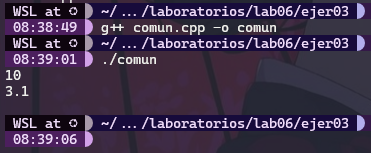
\includegraphics[width=0.5\textwidth]{img/Prueba03.png}
    \caption{Salida del programa al ejecutar el código proporcionado}
\end{figure}



\subsection {\textcolor{red}{Commits realizados}}

\subsubsection {Primer Commit}

\begin{itemize}
    \item En este primer commit se subió el código completo del ejercicio la implementación de la clase template para una lista enlazada simple en C++.
    \item Se incluyó el archivo main.cpp para probar la funcionalidad de la clase template
\end{itemize}

\begin{figure}[H]
    \centering
    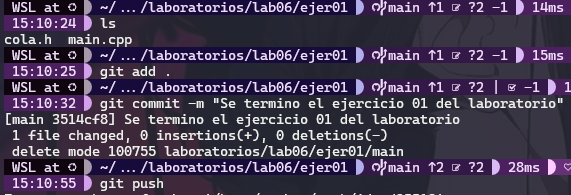
\includegraphics[width=0.8\textwidth]{img/Commit01.png}
    \caption{Primer Commit - Ejercicio 01 completo}
    \label{fig:commit1}
\end{figure}


\subsubsection {Segundo Commit}

\begin{itemize}
    \item En este segundo commit se subió el análisis del código brindado en la guía de laboratorio para el ejercicio 02.
    \item Se incluyó la explicación del comportamiento del código y la salida obtenida al ejecutarlo.
\end{itemize}

\begin{figure}[H]
    \centering
    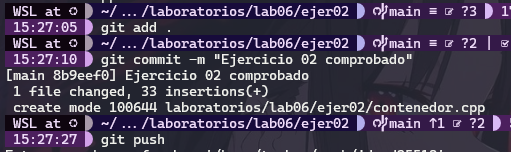
\includegraphics[width=0.8\textwidth]{img/Commit02.png}
    \caption{Segundo Commit - Ejercicio 02}
    \label{fig:commit2}
\end{figure}


\subsubsection {Tercer Commit}

\begin{itemize}
    \item En este tercer commit se subió el análisis del código brindado en la guía de laboratorio para el ejercicio 03.
    \item Se incluyó la explicación del comportamiento del código y la salida obtenida al ejecutarlo.
\end{itemize}

\begin{figure}[H]
    \centering
    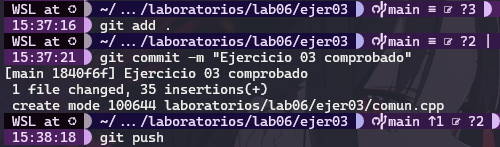
\includegraphics[width=0.8\textwidth]{img/Commit03.png}
    \caption{Tercer Commit - Ejercicio 03}
    \label{fig:commit3}
\end{figure}



\subsection {Estructura del laboratorio}

A continuación se muestra la estructura de archivos y carpetas del laboratorio realizado:
Claramente los archivos de compilación y otros que se pudieron generar no se subieron al repositorio.

\begin{figure}[H]
    \centering
    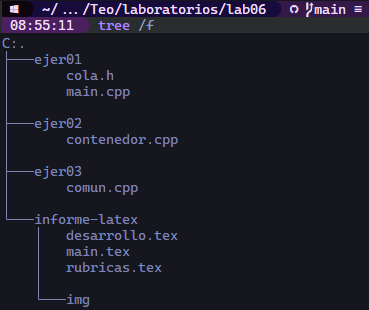
\includegraphics[width=0.6\textwidth]{img/Estructura.png}
    \caption{Estructura de archivos y carpetas del laboratorio}
    \label{fig:estructura}
\end{figure}



\section{Cuestionario}

\subsection{Revisar y encontrar diferencias, ventajas y desventajas entre plantillas y polimorfismo.}

\subsubsection{Diferencias}
\begin{itemize}
    \item Las plantillas permiten la creación de funciones y clases genéricas que pueden trabajar con cualquier tipo de dato, mientras que el polimorfismo permite que una función o método se comporte de manera diferente según el objeto que lo invoque.
    \item Las plantillas se resuelven en tiempo de compilación, generando código específico para cada tipo utilizado, mientras que el polimorfismo se resuelve en tiempo de ejecución mediante el uso de punteros o referencias a clases base.
\end{itemize}

\subsubsection{Ventajas}
\begin{itemize}
    \item Las plantillas permiten reutilizar código y evitar la duplicación, ya que una sola definición puede manejar múltiples tipos de datos.
    \item El polimorfismo permite la extensibilidad del código, ya que se pueden agregar nuevas clases derivadas sin modificar el código existente.
\end{itemize}

\subsubsection{Desventajas}
\begin{itemize}
    \item Las plantillas pueden aumentar el tamaño del código generado debido a la instanciación de múltiples versiones de la misma función o clase.
    \item El polimorfismo puede introducir una sobrecarga en tiempo de ejecución debido a la resolución dinámica de métodos.
\end{itemize}

\subsection{Revisar sobre funciones amigas, cómo se integra a las plantillas.}

Las funciones amigas en C++ son funciones que tienen acceso a los miembros privados y protegidos de una clase, incluso si no son miembros de esa clase. Para integrar funciones amigas con plantillas, se puede declarar una función amiga dentro de una clase plantilla utilizando la palabra clave `friend`. Esto permite que la función amiga pueda acceder a los miembros privados de cualquier instancia de la clase plantilla, independientemente del tipo de dato utilizado. \\

Aquí se presenta un ejemplo de cómo declarar una función amiga en una clase plantilla:
\begin{lstlisting}[style=cpp-style, caption={Función amiga en una clase plantilla}]
template <typename T>
class MiClase {
    T dato;
public:
    MiClase(T val) : dato(val) {}
    friend void mostrarDato<>(const MiClase<T>& obj);
};
template <typename T>
void mostrarDato(const MiClase<T>& obj) {
    std::cout << "Dato: " << obj.dato << std::endl;
}
\end{lstlisting}



